\section{Problem 2}
\label{problem2}
\subsection{Question}
\vspace*{10pt}
Write a Python program that:
\begin{enumerate}
\item takes as a command line argument a web page
\item extracts all the links from the page
\item lists all the links that result in PDF files, and prints out
      the bytes for each of the links.  (note: be sure to follow
      all the redirects until the link terminates with a "200 OK".)
\item show that the program works on 3 different URIs, one of which
needs to be:\\
http://www.cs.odu.edu/\~{}mln/teaching/cs532-s16/test/pdfs.html
\end{enumerate}
 
\subsection{Answer}
\vspace*{5mm}
In this python program, modules that are being used: 
\begin{enumerate}
\item Beautiful Soup is an HTML/XML parser for Python that can turn even invalid markup into a parse tree. It provides simple, idiomatic ways of navigating, searching, and modifying the parse tree.\cite{bs4} 
\\
\item Validators can be any callable that takes a single parameter which checks the new value before it is assigned to the attribute. Validators are permitted to modify a received value so that it is appropriate for the attribute definition. For example, using int as a validator will cast a correctly formatted string to a number, or raise an exception if it can not. However. the correct way to use a validator that ensure the correct type is to use the Type validator.\cite{validators}
\\
\item Requests takes all of the work out of Python HTTP/1.1 — making your integration with web services seamless. There’s no need to manually add query strings to your URLs, or to form-encode your POST data. Keep-alive and HTTP connection pooling are 100\% automatic, powered by urllib3, which is embedded within Requests.\cite{requests}
\end{enumerate}

\newpage
\vspace*{5pt}
\begin{center}
	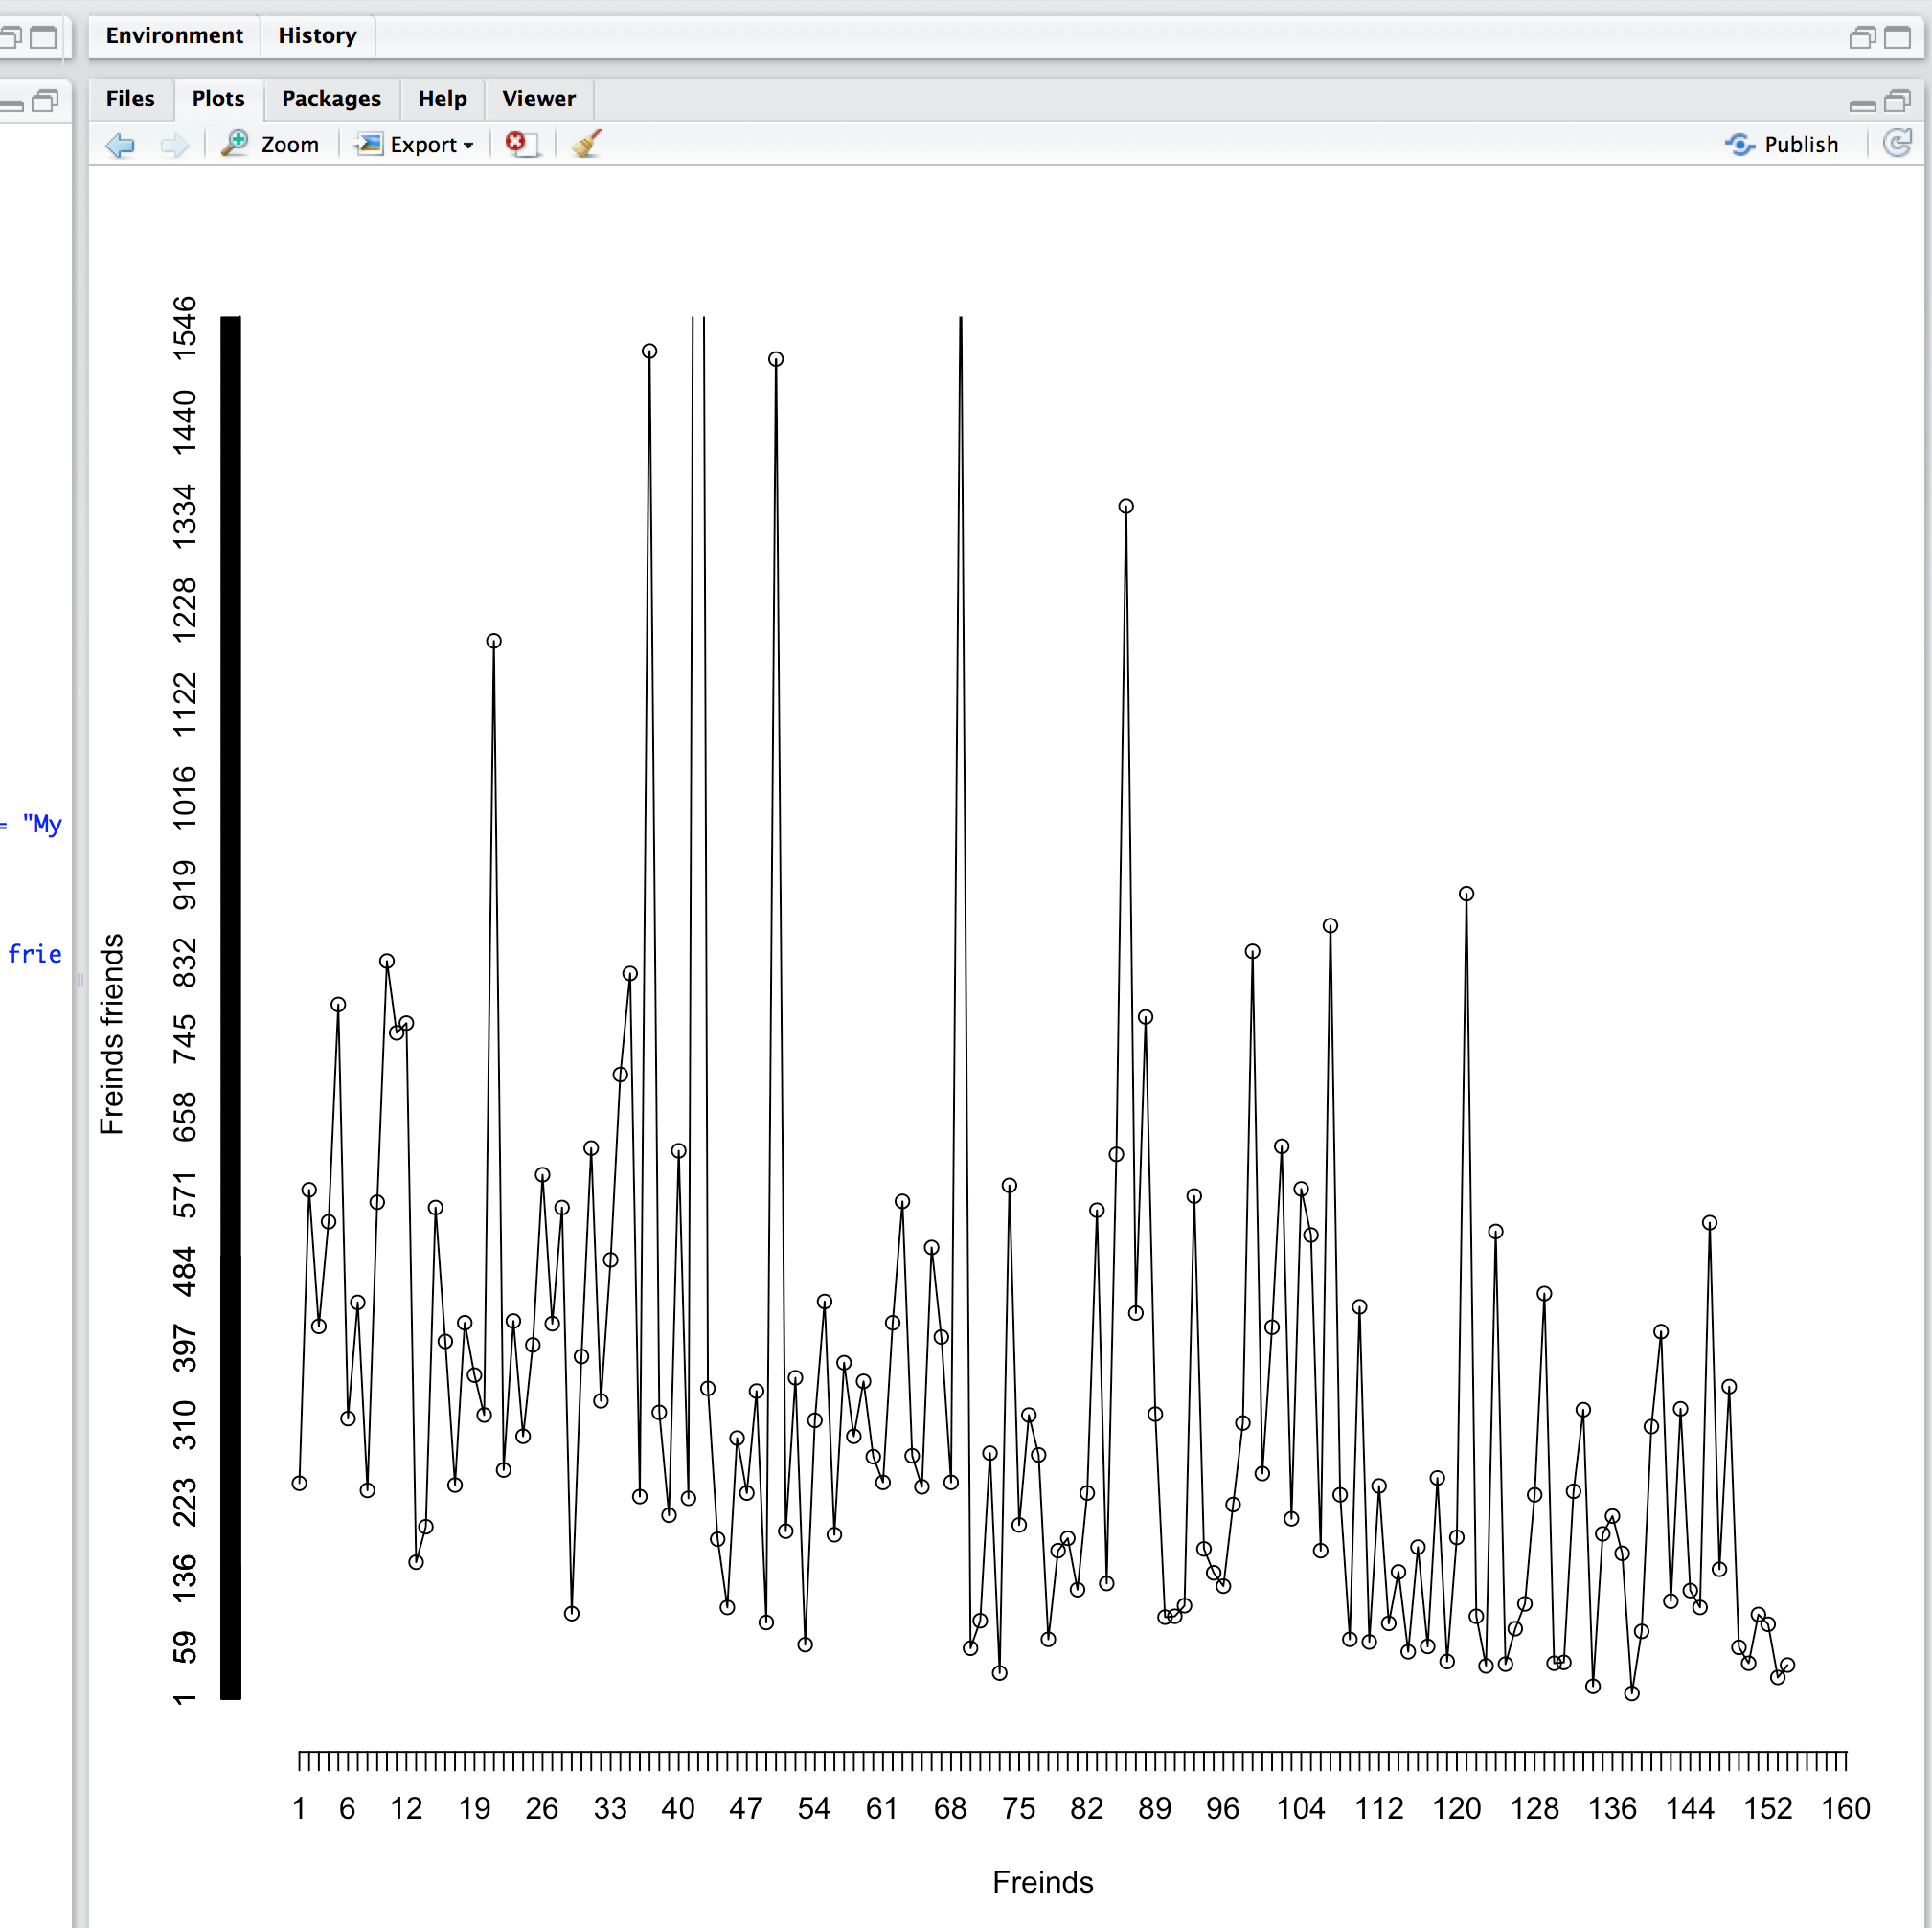
\includegraphics[scale=0.85]{Q2/fig1.png}
	\centerline{\textit{Figure 6: Output of q2.py at http://www.cs.odu.edu/\~{}mln/teaching/cs532-s16/test/pdfs.html
}}
\end{center}
\vspace*{5pt}
\begin{center}
	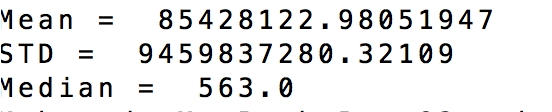
\includegraphics[scale=0.85]{Q2/fig2.png}
	\centerline{\textit{Figure 7: Output of q2.py at https://ws-dl.cs.odu.edu/Main/Pubs}}
\end{center}
\vspace*{5mm}
\begin{center}
	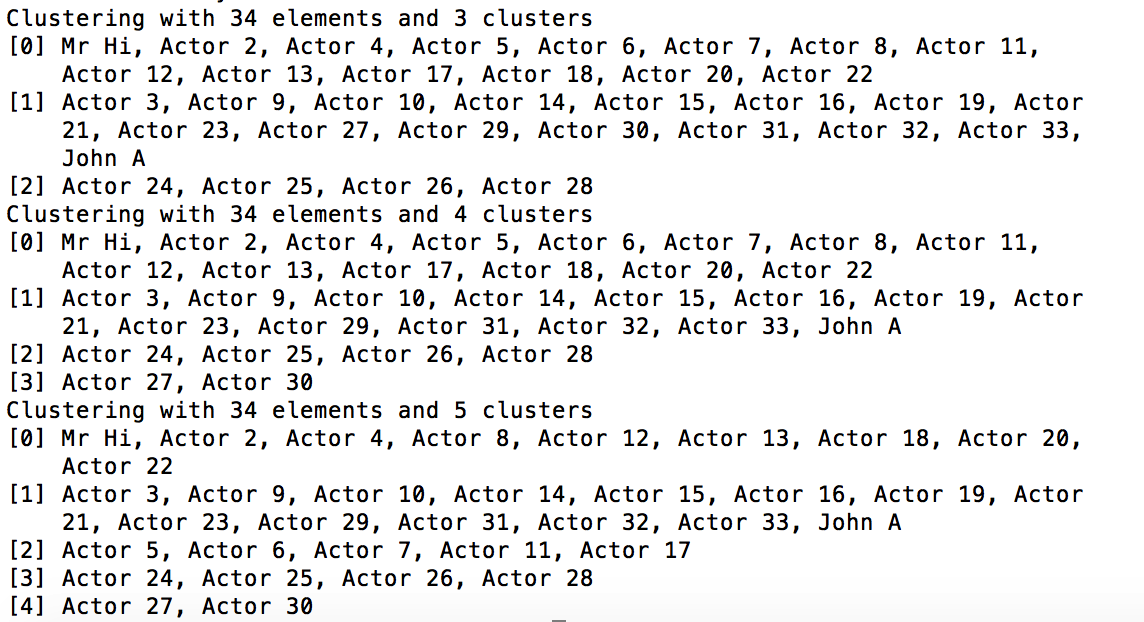
\includegraphics[scale=0.70]{Q2/fig3.png}
	\centerline{\textit{Figure 8: Output of q2.py at http://odu.edu/admission/graduate}}
\end{center}
Following python program $q2.py$, which accepts URL as argument and extracts PDF's from from the link:
\vspace*{1mm}

\begin{lstlisting}[frame = single,breaklines=true,numbers=left]
import sys
import requests
import validators
import locale
from urllib.parse import urlparse
from bs4 import BeautifulSoup

def main(url):
    print('\nExtracting all pdf links from: %s' % url)

    if requests.get(url).status_code != 200:
        print('\nURL not Found!\n')
        return
    page = requests.get(url).text
    url = 'http://' + urlparse(url).netloc
	
    soup = BeautifulSoup(page, 'html.parser')
    all_links = []
    for link in soup.find_all('a'):
        urls = link.get('href')
        if ((len(urls) > 6 and urls[:7].lower() != 'http://') 
        or len(urls) < 7) and urls[:8].lower() != 'https://':
            if urls[:2] == '//':
                urls = 'http:' + urls
            elif urls[0] != '/':    
                urls = url + '/' + urls
            else:
                urls = url + urls

        try:
            r = requests.get(urls)
            if 'Content-Type' in r.headers and 
            r.headers['Content-Type'] == 'application/pdf':
                if r.status_code == 200:
                    try:
                        all_links.append((urls, 
                        r.headers['Content-Length']))
                    except KeyError:
                        r.headers['Content-Length'] = '???'
                        all_links.append((urls, 
                        r.headers['Content-Length']))
        except requests.exceptions.SSLError:
            print('Couldn\'t open: %s. 
            URL requires authentication.' % urls)
        except requests.exceptions.ConnectionError:
            print('Couldn\'t open: %s. Connection refused.' % urls)
    print('\nList of all PDFs Links:')
    pdf_links = set(all_links)
    all_links = list(pdf_links)
    if len(all_links) > 0:
        for i in range(len(pdf_links)):
            if all_links[i][1] == '???':
                print('%s, File Size: %s bytes \n'
                 % (all_links[i][0], all_links[i][1]))
            else:
                print('%s, File Size: %s bytes \n' 
                % (all_links[i][0],                                  
                locale.format("%d", int(all_links[i][1]),
                grouping=True)))
    else:
        print('\nNo PDFs links for above URI.')
    return
if __name__ == '__main__':
    if len(sys.argv) != 2:
        print('\nUsage: python q2.py [url]')
        sys.exit(-1)
    if not validators.url(sys.argv[1]):
        print('URL is Invalid, Please try again')
        sys.exit(1)
    main(sys.argv[1])
    sys.exit(0)
\end{lstlisting}

